%%%%%%%%%%%%%%%%%%%%%%%%%%%%%%%%%%%%%%%%%%%%%%%%%%%%%%%%%%%%%%%%%%%%%%%%%%%%%%%
% Sample LaTeX format for a University of Arizona thesis
%
% Jeff Rodriguez
% jjrodrig@email.arizona.edu
%%%%%%%%%%%%%%%%%%%%%%%%%%%%%%%%%%%%%%%%%%%%%%%%%%%%%%%%%%%%%%%%%%%%%%%%%%%%%%%

\documentclass[PhD,copyright]{uathesis} % options: MS,PhD,draft,copyright,twoside

\usepackage{epsfig} \psfull
\usepackage{graphicx}
%\usepackage{amsmath}
%\usepackage{url}
%\usepackage{natbib}

% Edit the following lines to match the file names of your chapters.
\newcommand{\allthefiles}
{preface,intro,bg,theory,results,concl,details,refs}

\begin{document}

% Note:  preface.tex contains "[Limited to 150 words for an M.S. thesis and 350 words for a Ph.D. dissertation.]
The applications of electric and magnetic fields are widespread.
The goal of this work was to develop the mathematical foundations for static
fields.
Four basic laws are presented which describe the relationships between the
electric flux density, the electric charge density, the electric field
intensity, the magnetic field intensity, the electric current density, and the
magnetic flux density.
A detailed derivation of the corresponding equations is presented, along with a
discussion of their applications.
Experimental results are also shown, which confirm the validity of the
theoretical work.
"
\SgSetTitle{DATA AND DOMAIN UNCERTAINTY IN MACHINE LEARNING}
\SgSetAuthor{Artin Majdi}
\SgSetAuthorDegrees{M.Sc.}
\SgSetYear{2023}
\SgSetDegree{Doctor of Philosophy}
\SgSetDepartment{Electrical \& Computer Engineering}
\SgSetUniversity{University of Arizona}
\SgSetDeclarationDate{June, 2023}
\SgSetSupervisor{Jeff J. Rodriguez}
\SgSetSuperTitle{Professor}
\SgSetSuperDept{Electrical and Computer Engineering}
\SgSetSecondMember{Carlos Alsua}
\SgSetThirdMember{Ali Bilgin}
\SgSetFourthMember{Greg Ditzler}
%
\fancyhf{}
\cfoot{\thepage}
\chead{\th}
%
\SgAddTitle%
\SgAddApproval%
\SgAddStatement%
%
\begin{acknowledgments}
I would like to express my sincere gratitude to my supervisor,
Dr.\ Carl F.\ Gauss, for the suggestion of this research topic and for his
guidance and support throughout this project.
Thanks are also extended to Dr.\ Charles A. Coulomb and Dr.\ Conte A. Volta
for their participation on the committee and for their helpful comments.
My fellow graduate students, Mr.\ Andre M. Ampere, Mr.\ Georg S. Ohm, and
Mr.\ Michael Faraday, deserve many thanks for their friendship and help during
my graduate studies.
I would like to thank the members of my family, who have always supported my
education with their love, encouragement, patience, and support.
Finally, thanks to the German Electric Power Company for funding my research
assistantship.
\end{acknowledgments}
% \begin{dedication}
% To my wife, Bertha,\\
% whose love and encouragement\\
% made this possible
% \end{dedication}
%
\SgAddToc%  Table of contents.
\SgAddLof%  List of figures.
\SgAddLot%  List of tables.
\SgAddLoa%  List of algorithms.
	% title page, statement by author, ..., list of tables
%%%%%%%%%%%%%%%%%%%%%%%%%%%%%%%%%%%%%%%%%%%%%%%%%%%%%%%%%%%%%%%%%%%%%%%%%%%%%%%
\chapter{Introduction}
%%%%%%%%%%%%%%%%%%%%%%%%%%%%%%%%%%%%%%%%%%%%%%%%%%%%%%%%%%%%%%%%%%%%%%%%%%%%%%%

% Be sure to carefully read the IEEE Editorial Style Manual,
% http://www.ieee.org/documents/style_manual.pdf

This is the introduction.  This is the introduction.  This is the introduction.
This is the introduction.  This is the introduction.  This is the introduction.
This is the introduction.  This is the introduction.  This is the introduction.

This is the introduction.  This is the introduction.  This is the introduction.
This is the introduction.  This is the introduction.  This is the introduction.
This is the introduction.  This is the introduction.  This is the introduction.
		% introduction
%%%%%%%%%%%%%%%%%%%%%%%%%%%%%%%%%%%%%%%%%%%%%%%%%%%%%%%%%%%%%%%%%%%%%%%%%%%%%%%
\chapter{Background}
%%%%%%%%%%%%%%%%%%%%%%%%%%%%%%%%%%%%%%%%%%%%%%%%%%%%%%%%%%%%%%%%%%%%%%%%%%%%%%%

Background background background background background background background
background background background background background background background
background background background background background.

%%%%%%%%%%%%%%%%%%%%%%%%%%%%%%%%%%%%%%%%%%%%%%%%%%%%%%%%%%%%%%%%%%%%%%%%%%%%%%%
\section{Vector Calculus}
%%%%%%%%%%%%%%%%%%%%%%%%%%%%%%%%%%%%%%%%%%%%%%%%%%%%%%%%%%%%%%%%%%%%%%%%%%%%%%%

Vector calculus vector calculus vector calculus vector calculus vector
calculus vector calculus vector calculus vector calculus vector calculus
vector calculus vector calculus vector calculus vector calculus.

%%%%%%%%%%%%%%%%%%%%%%%%%%%%%%%%%%%%%%%%%%%%%%%%%%%%%%%%%%%%%%%%%%%%%%%%%%%%%%%
\subsection{Gradient}
%%%%%%%%%%%%%%%%%%%%%%%%%%%%%%%%%%%%%%%%%%%%%%%%%%%%%%%%%%%%%%%%%%%%%%%%%%%%%%%

Gradient gradient gradient gradient gradient gradient gradient gradient
gradient gradient gradient gradient gradient gradient gradient gradient
gradient gradient gradient gradient gradient gradient gradient gradient.

%%%%%%%%%%%%%%%%%%%%%%%%%%%%%%%%%%%%%%%%%%%%%%%%%%%%%%%%%%%%%%%%%%%%%%%%%%%%%%%
\subsection{Divergence}
%%%%%%%%%%%%%%%%%%%%%%%%%%%%%%%%%%%%%%%%%%%%%%%%%%%%%%%%%%%%%%%%%%%%%%%%%%%%%%%

Divergence divergence divergence divergence divergence divergence divergence
divergence divergence divergence divergence divergence divergence divergence
divergence divergence divergence divergence divergence divergence divergence.

%%%%%%%%%%%%%%%%%%%%%%%%%%%%%%%%%%%%%%%%%%%%%%%%%%%%%%%%%%%%%%%%%%%%%%%%%%%%%%%
\subsection{Curl}
%%%%%%%%%%%%%%%%%%%%%%%%%%%%%%%%%%%%%%%%%%%%%%%%%%%%%%%%%%%%%%%%%%%%%%%%%%%%%%%

Curl curl curl curl curl curl curl curl curl curl curl curl curl curl curl
curl curl curl curl curl curl curl curl curl curl curl curl curl curl curl
curl curl curl curl curl curl curl curl curl curl curl curl curl curl curl.

%%%%%%%%%%%%%%%%%%%%%%%%%%%%%%%%%%%%%%%%%%%%%%%%%%%%%%%%%%%%%%%%%%%%%%%%%%%%%%%
\section{Electricity and Magnetism}
%%%%%%%%%%%%%%%%%%%%%%%%%%%%%%%%%%%%%%%%%%%%%%%%%%%%%%%%%%%%%%%%%%%%%%%%%%%%%%%

Electricity electricity electricity electricity electricity electricity
electricity electricity electricity electricity electricity electricity
electricity electricity electricity electricity electricity electricity.
		% background
%%%%%%%%%%%%%%%%%%%%%%%%%%%%%%%%%%%%%%%%%%%%%%%%%%%%%%%%%%%%%%%%%%%%%%%%%%%%%%%
\chapter{A New Theory of Electromagnetics}
%%%%%%%%%%%%%%%%%%%%%%%%%%%%%%%%%%%%%%%%%%%%%%%%%%%%%%%%%%%%%%%%%%%%%%%%%%%%%%%

New mathematical relationships have been derived,
fundamental behavior of electrostatie and steady magnetic fields.
These equations were verified by experimental results, as discussed in
Chap. \ref{ch-results}.
Portions of this work are based on earlier results by Gauss \cite{Gauss},
Ampere \cite{Ampere}, and Faraday \cite{Faraday}.

%%%%%%%%%%%%%%%%%%%%%%%%%%%%%%%%%%%%%%%%%%%%%%%%%%%%%%%%%%%%%%%%%%%%%%%%%%%%%%%
\section{Electric Flux Density}
%%%%%%%%%%%%%%%%%%%%%%%%%%%%%%%%%%%%%%%%%%%%%%%%%%%%%%%%%%%%%%%%%%%%%%%%%%%%%%%

Eq. \ref{eq-gauss} is the first of Maxwell's equations, which describes the
relationship between the electric flux density and the electric charge density.
\begin{equation}
\vec{\nabla} \cdot \vec{D} = \rho
\label{eq-gauss}
\end{equation}
This is derived from the point form of Gauss's Law, given in integral form as
\begin{equation}
\oint_S \vec{D} \cdot d\vec{S} = Q
\end{equation}

%%%%%%%%%%%%%%%%%%%%%%%%%%%%%%%%%%%%%%%%%%%%%%%%%%%%%%%%%%%%%%%%%%%%%%%%%%%%%%%
\section{Electric Field Intensity}
%%%%%%%%%%%%%%%%%%%%%%%%%%%%%%%%%%%%%%%%%%%%%%%%%%%%%%%%%%%%%%%%%%%%%%%%%%%%%%%

Eq. \ref{eq-amp} shows the second of Maxwell's equations, which involves the
electric field intensity.
\begin{equation}
\vec{\nabla} \times \vec{E} = 0
\label{eq-amp}
\end{equation}
This is related to the point form of Ampere's Circuital Law,
\begin{equation}
\oint \vec{H} \cdot d\vec{L} = I
\end{equation}

%%%%%%%%%%%%%%%%%%%%%%%%%%%%%%%%%%%%%%%%%%%%%%%%%%%%%%%%%%%%%%%%%%%%%%%%%%%%%%%
\section{Magnetic Field Intensity}
%%%%%%%%%%%%%%%%%%%%%%%%%%%%%%%%%%%%%%%%%%%%%%%%%%%%%%%%%%%%%%%%%%%%%%%%%%%%%%%

The third of Maxwell's equations describes the relationship between the
magnetic field intensity and the electric current density:
\begin{equation}
\vec{\nabla} \times \vec{H} = \vec{J}
\end{equation}
The corresponding integral formula is
\begin{equation}
\oint \vec{H} \cdot d\vec{L} = I
\end{equation}

%%%%%%%%%%%%%%%%%%%%%%%%%%%%%%%%%%%%%%%%%%%%%%%%%%%%%%%%%%%%%%%%%%%%%%%%%%%%%%%
\section{Magnetic Flux Density}
%%%%%%%%%%%%%%%%%%%%%%%%%%%%%%%%%%%%%%%%%%%%%%%%%%%%%%%%%%%%%%%%%%%%%%%%%%%%%%%

The last of Maxwell's equations involves the magnetic flux density:
\begin{equation}
\vec{\nabla} \times \vec{B} = 0
\end{equation}
The corresponding integral formula is
\begin{equation}
\oint_S \vec{B} \cdot d\vec{S} = 0
\end{equation}
	% description of new theory
%%%%%%%%%%%%%%%%%%%%%%%%%%%%%%%%%%%%%%%%%%%%%%%%%%%%%%%%%%%%%%%%%%%%%%%%%%%%%%%
\chapter{Experimental Results}
\label{ch-results}
%%%%%%%%%%%%%%%%%%%%%%%%%%%%%%%%%%%%%%%%%%%%%%%%%%%%%%%%%%%%%%%%%%%%%%%%%%%%%%%

This chapter describes the experiments that were performed, along with the
results of the experiments that were performed when they were performed.
Experiments were performed experiments were performed
Experiments were performed experiments were performed
Experiments were performed experiments were performed.

%%%%%%%%%%%%%%%%%%%%%%%%%%%%%%%%%%%%%%%%%%%%%%%%%%%%%%%%%%%%%%%%%%%%%%%%%%%%%%%
\section{Experimental Setup}
%%%%%%%%%%%%%%%%%%%%%%%%%%%%%%%%%%%%%%%%%%%%%%%%%%%%%%%%%%%%%%%%%%%%%%%%%%%%%%%

Fig. \ref{fig-nifty} shows a nifty PostScript drawing.
Experimental setup experimental setup experimental setup experimental setup
experimental setup experimental setup experimental setup experimental setup
experimental setup experimental setup experimental setup experimental setup
experimental setup experimental setup experimental setup experimental setup
experimental setup experimental setup experimental setup experimental setup.
\begin{figure}
\smallskip
\centerline{\epsfig{file=fig-nifty.eps,width=5.0in,height=2in}}
\smallskip
\caption{Nifty PostScript drawing.}
\label{fig-nifty}
\smallskip
\end{figure}

%%%%%%%%%%%%%%%%%%%%%%%%%%%%%%%%%%%%%%%%%%%%%%%%%%%%%%%%%%%%%%%%%%%%%%%%%%%%%%%
\section{Presentation of Data}
%%%%%%%%%%%%%%%%%%%%%%%%%%%%%%%%%%%%%%%%%%%%%%%%%%%%%%%%%%%%%%%%%%%%%%%%%%%%%%%

Various measurements were made and data was tabulated.
Table \ref{table-data} gives a presentation of the data.
Presentation of data presentation of data presentation of data.
Presentation of data presentation of data presentation of data.
Presentation of data presentation of data presentation of data.
Presentation of data presentation of data presentation of data.
\begin{table}
\smallskip
\begin{center}
\begin{tabular}{|l|c|c|}
\hline
Experiment & Measurement (units) \\
\hline
1	&	10.3 \\
\hline
2	&	23.5 \\
\hline
3	&	42.9 \\
\hline
\end{tabular}
\end{center}
\smallskip
\caption{Experimental Data}
\label{table-data}
\smallskip
\end{table}

%%%%%%%%%%%%%%%%%%%%%%%%%%%%%%%%%%%%%%%%%%%%%%%%%%%%%%%%%%%%%%%%%%%%%%%%%%%%%%%
\section{Analysis of Results}
%%%%%%%%%%%%%%%%%%%%%%%%%%%%%%%%%%%%%%%%%%%%%%%%%%%%%%%%%%%%%%%%%%%%%%%%%%%%%%%

Several observations about the experimental results will now be made.
Analysis of results analysis of results analysis of results
analysis of results analysis of results analysis of results
analysis of results analysis of results analysis of results
analysis of results analysis of results analysis of results.
	% experimental results
%%%%%%%%%%%%%%%%%%%%%%%%%%%%%%%%%%%%%%%%%%%%%%%%%%%%%%%%%%%%%%%%%%%%%%%%%%%%%%%
\chapter{Conclusion}
%%%%%%%%%%%%%%%%%%%%%%%%%%%%%%%%%%%%%%%%%%%%%%%%%%%%%%%%%%%%%%%%%%%%%%%%%%%%%%%

This is the conclusion.  This is the conclusion.  This is the conclusion.
This is the conclusion.  This is the conclusion.  This is the conclusion.
This is the conclusion.  This is the conclusion.  This is the conclusion.

This is the conclusion.  This is the conclusion.  This is the conclusion.
This is the conclusion.  This is the conclusion.  This is the conclusion.
This is the conclusion.  This is the conclusion.  This is the conclusion.
		% conclusion
\appendix		% begin appendix mode
%%%%%%%%%%%%%%%%%%%%%%%%%%%%%%%%%%%%%%%%%%%%%%%%%%%%%%%%%%%%%%%%%%%%%%%%%%%%%%%
\chapter{Detailed Material}
%%%%%%%%%%%%%%%%%%%%%%%%%%%%%%%%%%%%%%%%%%%%%%%%%%%%%%%%%%%%%%%%%%%%%%%%%%%%%%%

Here we present the gruesome details of the derivations of some equations.
Here we present the gruesome details of the derivations of some equations.
Here we present the gruesome details of the derivations of some equations.

Here we present the gruesome details of the derivations of some equations.
Here we present the gruesome details of the derivations of some equations.
Here we present the gruesome details of the derivations of some equations.
	% detailed material
%%%%%%%%%%%%%%%%%%%%%%%%%%%%%%%%%%%%%%%%%%%%%%%%%%%%%%%%%%%%%%%%%%%%%%%%%%%%%%%
\begin{thebibliography}{99}
%%%%%%%%%%%%%%%%%%%%%%%%%%%%%%%%%%%%%%%%%%%%%%%%%%%%%%%%%%%%%%%%%%%%%%%%%%%%%%%

% For further info regarding the IEEE bibliography style, see
% http://www.ieee.org/documents/ieeecitationref.pdf

% Book with one author
\bibitem{Ampere}
A. M. Ampere, \emph{Electricity and Magnetism}.
Englewood Cliffs, NJ: Prentice Hall, 1989.

% Book with two authors
\bibitem{Baker}
A. B. Baker and C. D. Brooks, \emph{Electricity and Magnetism}.
Englewood Cliffs, NJ: Prentice Hall, 1989.

% Book with three authors
\bibitem{Coulomb}
C. A. Coulomb, A. B. Carter, and C. D. Chang,
\emph{Electricity and Magnetism}.
Englewood Cliffs, NJ: Prentice Hall, 1989.

% Book with more than three authors
\bibitem{Dickens}
A. B. Dickens \emph{et al.}, \emph{Electricity and Magnetism}.
Englewood Cliffs, NJ: Prentice Hall, 1989.

% A later edition
\bibitem{Edison}
T. A. Edison, \emph{Electricity and Magnetism}, 2nd ed.
Englewood Cliffs, NJ: Prentice Hall, 1989.

% Part of a multiple-volume set
\bibitem{Faraday}
M. Faraday, \emph{Electricity and Magnetism}, vol. 2.
Englewood Cliffs, NJ: Prentice Hall, 1989.

% A book with one editor
\bibitem{Gauss}
C. F. Gauss, Ed., \emph{Electricity and Magnetism}.
Englewood Cliffs, NJ: Prentice Hall, 1989.

% A book with more than one editor
\bibitem{Henry}
J. Henry and A. B. Hartman, Eds., \emph{Electricity and Magnetism}.
Englewood Cliffs, NJ: Prentice Hall, 1989.

% A selection from an edited book
\bibitem{Ingram}
A. B. Ingram, ``Theoretical Analysis of Electromagnetics,"
in \emph{Electricity and Magnetism}, B. C. Ivanhoe, Ed.
Englewood Cliffs, NJ: Prentice Hall, 1989, pp. 123--145.

% A reprint of an article originally appearing in a journal
\bibitem{Jones}
A. B. Jones, ``Theoretical Analysis of Electromagnetics,"
in \emph{Electricity and Magnetism}, C. D. Johnson, Ed.
Englewood Cliffs, NJ: Prentice Hall, 1989, pp. 123--145.
Reprinted from \emph{IEEE Trans. on Electromagnetics},
vol. 10, Jan. 1989, pp. 323--345.

% A journal article
\bibitem{Kaiser}
A. B. Kaiser, ``Theoretical Analysis of Electromagnetics,"
\emph{IEEE Trans. on Electromagnetics}, vol. 10, Jan. 1989, pp. 123--145.

% An article in a conference proceedings
\bibitem{Leibniz}
G. W. Leibniz, ``Theoretical Analysis of Electromagnetics,"
in \emph{Proc. Intl. Conf. on Electromagnetics}, 1989, pp. 123--145.

% An article in a SPIE conference proceedings
\bibitem{Maxwell}
J. C. Maxwell, ``Theoretical Analysis of Electromagnetics,"
in \emph{Electricity and Magnetism}, A. B. Moore, Ed., Proc. of SPIE,
vol. 10, 1989, pp. 123--145.

% An article to be submitted to a journal for publication
\bibitem{Newton}
I. Newton, ``Theoretical Analysis of Electromagnetics,"
\emph{IEEE Trans. on Electromagnetics}, in preparation.

% An article that has been submitted to a journal but not yet accepted
\bibitem{Ohm}
G. S. Ohm, ``Theoretical Analysis of Electromagnetics,"
\emph{IEEE Trans. on Electromagnetics}, submitted.

% An article that has been accepted to a journal but not yet printed
\bibitem{Parker}
A. B. Parker, ``Theoretical Analysis of Electromagnetics,"
\emph{IEEE Trans. on Electromagnetics}, accepted for publication.

% A thesis
\bibitem{Quinn}
A. B. Quinn, \emph{Electricity and Magnetism}.
M.S. thesis, Dept. of Electrical and Computer Engineering,
The Univ. of Arizona (Tucson), Dec. 1989.

% A dissertation
\bibitem{Roth}
A. B. Roth, \emph{Electricity and Magnetism}.
Ph.D. dissertation, Dept. of Electrical and Computer Engineering,
The Univ. of Arizona (Tucson), Dec. 1989.

% A technical report
\bibitem{Smith}
A. B. Smith, \emph{Electricity and Magnetism}.
Tech. report 123, Dept. of Electrical Engineering,
Rice Univ. (Houston, TX), Jan. 1989.

% A pamphlet or government document
\bibitem{TRC}
Southwest Research Council, \emph{Trends in Electromagnetics Research}.
Tucson, AZ: Southwest Research Council, 1989.

% Personal communication such as a personal letter or telephone call
\bibitem{Unser}
A. B. Unser, Dept. of Electrical Engineering, Rice Univ. (Houston, TX),
personal communication, Jan. 1989.

\end{thebibliography}
		% references

% Here's an alternative to the \thebibliography environment.
% \bibliographystyle{IEEEtran}
% \bibliography{Master}

% The following line generates a special abstract page, which may be needed
% for filing the dissertation with UMI.
% \makeumiabstract

\end{document}
